\documentclass{article}

\usepackage{amsmath}
\usepackage{graphicx}

\begin{document}

\newpage{}
\tableofcontents
\newpage{}

\newpage
\section{Jerarquia de Memoria}

La Jerarquia de Memoria, toma las ventajas del principio de localidad y el costo de performance de las memorias.
El principio de localidad dice que los programas no acceden al todo el codigo o datos uniformemente.

Tipico nivel de Jerarquia:

    \begin{figure}[h!]
        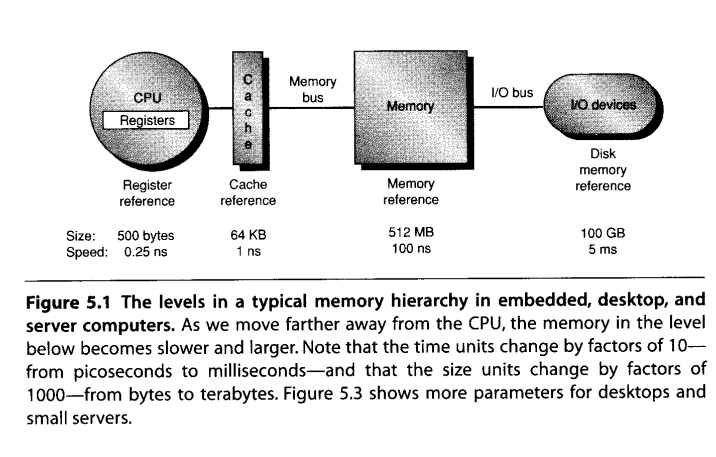
\includegraphics[width=\linewidth]{imagenes/Jeraquia_Memoria.png}
    \end{figure}
      

Como la memorias rapidas son caras, la Jerarquia de Memoria esta organizada en distitos niveles.

El objetivo es proveer un sistema de memoria con costos tan bajos como el nivel de memoria mas barato y
velocidad casi tan tapidos como el nivel mas veloz.

\subsection{Review Caches}
A continuación algunos terminos utilizados:

\textbf{Cache}: Es el primer nivel de la Jerarquia. 
\begin{enumerate}
\item Se utiliza cuando sea necesario un buffer para reusar items que ocurren comunmente.
\end{enumerate}

\textbf{Cache Hit}: Cuando la CPU requiere un dato y lo cuentra como item en la cache.

\textbf{Cache Miss}: Cuando la CPU requiere un dato y NO lo cuentra como item en la cache.
\begin{enumerate}
\item El tiempo requerido depende de la latencia y el ancho de banda de la memoria.
\item Es manejado por el hardware.
\end{enumerate}

\textbf{Bloque}: Una coleccion de datos con tamaño fijo que contiene la palabra requerida, es recuperada
de memoria y situada en la cache.

\textbf{Localidad temporal}: Nos dice que podemos probablemente vamos a necesitar el mismo datos en un futuro cercano.
    Entonces es util dejarlo en la cache para utilizarlo rapidamente.

\textbf{Localidad espacial}: Nos dice que hay altas posibilidades de utilizar pronto otro dato del mismo bloque.

\textbf{Paginas}: Espacios de memoria separados en bloques de tamaño fijo. 
\begin{enumerate} 
    \item Una pagina puede recidir tanto en memoria como en disco.
    \item Cuando el CPU hace referencia a un item dentro de una pagina que no esta presente (not present) en la cache, or memoria principal, se produce un PAGE FAULT, y la pagina entera es movida del disco a memoria principal.
    \item Como los page fault toman mucho tiempo, estos se manejan por software y la CPU no se detiene(STALLED)
    \item La cache y la memoria principal tienen la misma relacion en memoria y en disco.
\end{enumerate}


\subsection{Perfomance de Cache}

Para evaluar la perfomance de la cache expandiremos el uso de la ecuación de CPU Excecution Time.

\textbf{Memory Stall Cycles}: Número de ciclos que necesita esperar la CPU para acceder a la memoria.

    \begin{equation}
    CPU exe = (CPU clock cycles + Memory Stall cycles ) * Clock cycle time.
    \end{equation}
    
Memory Stall cycles depende de la cantidad de misses y el costo por miss.

    \begin{equation}
        Memory Stall cycles = Number of Misses * Miss Penalty
    \end{equation}
    \begin{equation}
        Memory Stall cycles = IC * \frac{Misses}{Instruction} * Miss Penalty
    \end{equation}
    \begin{equation}
        Memory Stall cycles = IC * \frac{MemoryAccess}{Instruction} * MissRate * Miss Penalty
    \end{equation}


Donde IC es Instruction Count. 

En la ultima formula los componentes se pueden medir facilmente. La cantidad de instrucciones (\textbf{IC}) se puede medir
Para medir las referencias a memoria \textbf{MemoryAccess}), cada instrucción requeiere un acceso a memoria (Instruction Access) y 
dependiendo de la instrucción se cuentan los accesos a datos en memoria (Data Access).

Calculamos el \textbf{MissPenalty} como un promedio.

El componente \textbf{MissRate} es simplemente la fraccion entre los accesos a cache que resultaron en misses 
divido el numero de accesos totales


El calculo de \textbf{MemoryStallCycle} puede definirse en terminos de número de accesos a memoria por instrucción, \textit{miss penalty} para lectura y escritura, y el \textit{miss rate} para lectura y escritura:

\begin{align*}
Memory Stall clock cycles = &IC * Instr. de lectura * MissRate Lectura * MissPenaltyLectura + \\
&IC * Instr. de Escritura * MissRateEscritura * MissPenaltyEscritura
\end{align*}

Para simplificar la formula, combinamos las lecturas y escrituras y buscamos un promedio para el miss rate y el miss penalty de escritura y lectura.

\begin{equation}
    Memory Stall cycles = IC * \frac{MemoryAccess}{Instruction} * MissRate * Miss Penalty
\end{equation}

El miss rate es una de las medidas mas importantes de diseño de cache.


\subsection{Categorias de organizacion de Cache}

En la imagen de abajo se muestra las restricciones cuando se quiere situar un bloque en cache.


\begin{figure}[h!]
    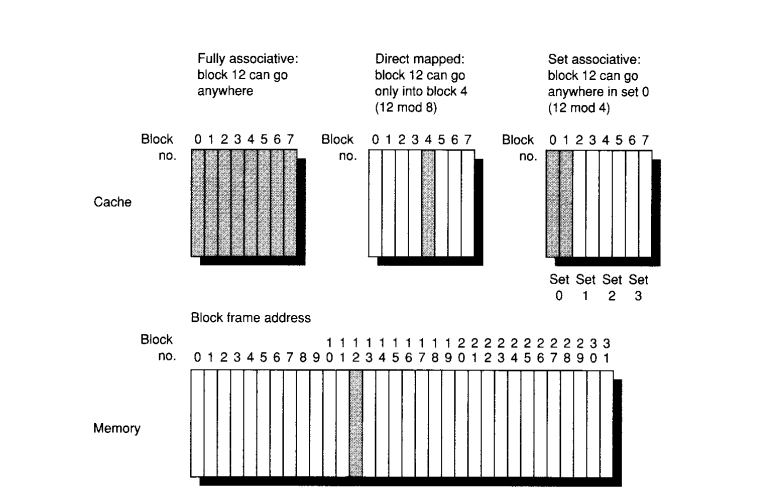
\includegraphics[width=\linewidth]{imagenes/CategoriasCache.png}
\end{figure}


\begin{itemize} 
    \item Si cada bloque tiene solo un lugar donde situarse en la cache, se dice que la cache es \textit{Direct Mapped}.
    \item Si cada bloque puede situarse en cualquier lugar de la cache, se dice que la cache es \textit{Fully Associative}.
    \item Si cada bloque puede situarse solo en algunos lugares restringidos de la cache, se dice que la cache es \textit{Set Associative}. Si hay N bloques en un conjunto se dice que la cache es \textit{N-Way Set Associative}.
\end{itemize}

\begin{figure}[h!]
    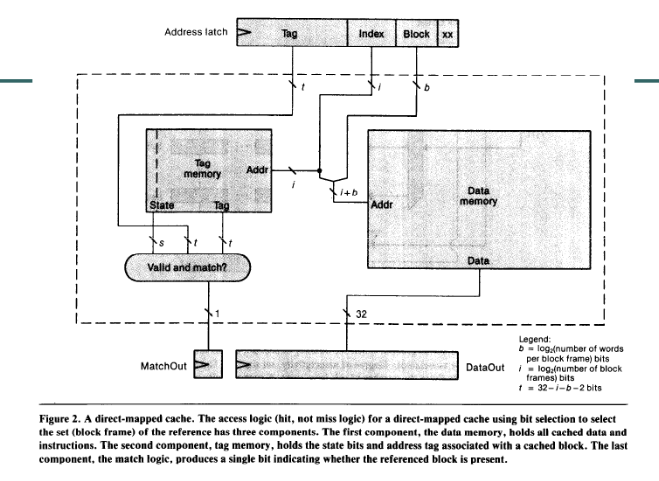
\includegraphics[width=\linewidth]{imagenes/CacheMapeoDirecto.png}
\end{figure}

\newpage

\begin{figure}[h!]
    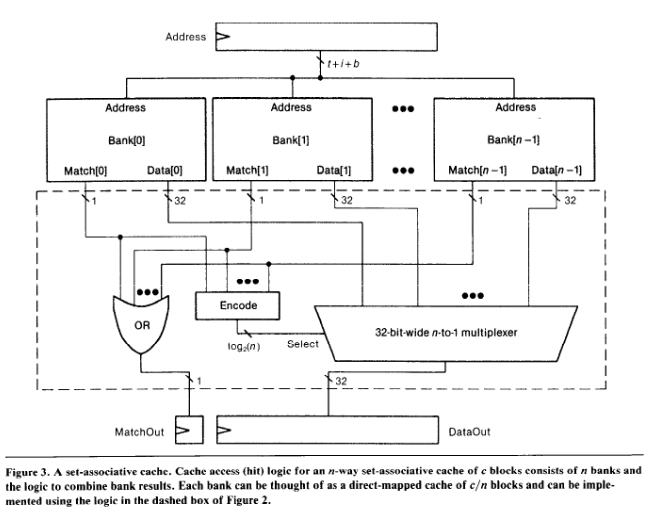
\includegraphics[width=\linewidth]{imagenes/CacheNWayAssosiative.png}
\end{figure}

\newpage

\subsection{¿Como se ubica un bloque en la Cache?}

La cache tiene un tag de direcciones (\textit{address tag}) en cada bloque de frame que te da la direccion del bloque (\textit{block address}).
El tag de cada bloque de cache debe tener toda la informacion necesario para validar si este coincide con la direccion del bloque provisto por la CPU.
Como regla todos los tags deben ser buscados en paralelo.


\begin{figure}[h!]
    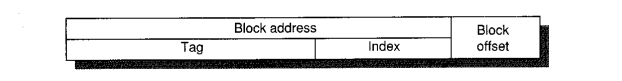
\includegraphics[width=\linewidth]{imagenes/DireccionVsCache.png}
\end{figure}

Para saber si el bloque de cache no tiene información valida se utiliza un bit de validez junto al tag para saber si o no contiene una dirección valida.

Exploremos la relación entra la dirección de la CPU (\textit{CPU Adress}) y la cache. La direccion se divide entre \textit{block address} y \textit{block offset}.
A su vez el el block address se puede dividir en \textit{tag field} y \textit{index field}. 
El block offset seleccionar el dato deseado dentro del bloque, el campo indice selecciona el conjunto, y el campo tag field es comparado con la porcion que corresponde de la dirección para buscar un hit. 

El indice es usado para seleccionar el conjunto. Pero el caso de unaa cache full asociativa, no tiene indice.

\subsection{¿Que bloque debe ser replazado ante un Cache Miss?}

Cuando un ocurre un cache miss, el controlador de la cache debe seleccionar un bloque para ser replazado con el dato deseado.
Para una cache \textit{direct map} el hardware requerido para la decision se simplifica ya que no requiere elección.
Con las caches \textit{full associative} y \textit{set associative} hay muchos bloques para elegir frente a un cache miss.
Hay tres estrategias para seleccionar que bloque remplazar:


\begin{itemize} 
    \item \textit{Random} - El bloque candidato es seleccionado aleatoriamente
    \item \textit{Least-recently used (LRU)} - Si el bloque recientemente usado es el mas probable para ser usado de nuevo, entonces un buen candidato para ser desechado es el bloque menos recientemente usado (\textit{the least-recently used block}).
    \item \textit{First in, first out(FIFO)} - Se remplaza por el bloque mas viejo. Es una aproximación a LRU ya que es complicado de implementar.
\end{itemize}

\subsection{¿Que pasa ante una escritura?}

Las lecturas dominan los accesos a cache del procesador. Todos los accesos son lecturas y muchas intrucciones no escriben en memoria. 
Haciendo que los casos comunes sean rapidos, estamos optimizando las caches para lecturas, especialmente cuando los procesadores
tradicionales esperan para completar una lectura pero no necesitan esperar por escrituras.

Los bloques pueden ser leidos de la cache al mismo tiempo que es leido el \textit{tag} y comparado. Entonces la parte solicitada del bloque es pasado al CPU inmediatamente.
Si la lectura es un miss, no hay un beneficio en este paralelismo.

Esta optimización no se puede realizar con escrituras. No se puede modificar un bloque hasta que se haya validado el tag para ver si la direccion es un hit. El chequeo del tag no puede hacerce en paralelo, ya que las escrituras normalmente llevan mas tiempo que las lecturas.
Otra complicación es que el procesador tambien especifica el tamaño del dato a escribir, usualmente entre 1 y 8 bytes; solo esa porción del bloque puede ser modificado. Al contrario que las lecturas, estas pueden acceder a mas bytes de los que son necesario.

Las politicas de escritura a menudo distingen dos diseños de cache.

\begin{itemize} 
    \item \textit{Write through} - La información es escrita en ambos bloques, en la cache y en el bloque de la memoria mas baja (\textit{lower-level memory}).
    \item \textit{Write back} - La información es escrita solo en el bloque de la cache. \textit{El bloque de cache modificado es escrito en memoria solo cuando esta es remplazada.}
\end{itemize}

Para reducir la frecuencia de remplazo de bloques con politica write back, se utiliza una marca de limpeza (\textbf{dirty bit}). El estado de este bit indica si el bloque esta \textit{dirty} (bloque modificado mientras estuvo en cache) o \textit{clean} (no fue modificado). Si esta marca esta en clean, no es necesario escribir el bloque en memoria ante un miss, porque la información contenida en el cache es identica al bloque encontrado en los niveles mas bajos.

Tanto write back y write through tienen sus \textit{ventajas}. Con write back las escrituras ocurren a la misma velocidad que la memoria cache, y si hay multiples escrituras dentro del bloque requerido, solo se requiere una escritura en el nivel mas bajo de memoria. Write back usa menos ancho de banda ya que no todas las escrituras van a memoria. Y tambien se ahorra energia al usar en menor medida el resto de la jerarquia de memoria y menos buses de memoria.

Write through es facil de implementar que write back. La cache siempre esta clean. Ademas tiene la ventaja de que el siguiente nivel de memoria mas bajo se tiene la copia del dato mas actualizado, lo cual se simplifica la coherencia de datos.

Dado que a veces el dato no es necesario en una escritura, hay dos opciones durante un \textit{write miss}

\begin{itemize} 
    \item \textit{Write allocate} - El bloque es alocado ante un write miss, seguido de un write hit por ensima. En este caso, \textit{el write miss actua como un read miss.}
    \item \textit{No-write allocate} - Ante un write miss, este no afecta la cache. El bloque es modificado solo en la memoria de nivel mas bajo.
\end{itemize}

Normalmente write back caches usa write allocate, suponiendo que el subsiguiente write al bloque sea capturado por la cache.
Write through cache se usa con no-write allocate y la razón es que si hay subsecuentes writes al bloque, los writes van a ir a la memoria de mas bajo nivel, y no hay ganancia al tenerlos cache. 


\subsection{Un ejemplo: Alpha 21264 Data Cache}

La cache contiene 64 Kbytes de datos y 64 bytes por bloque.

\begin{figure}[h!]
    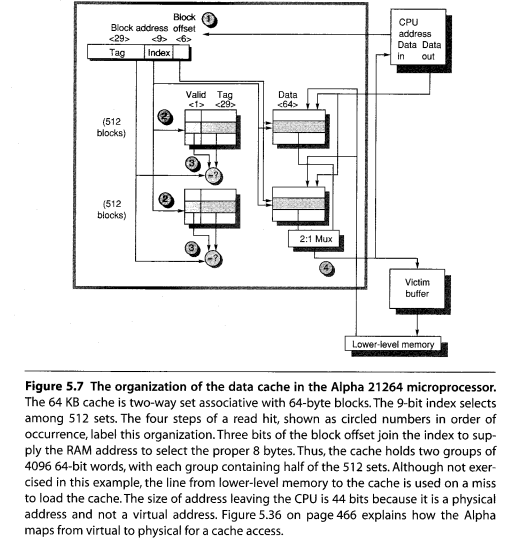
\includegraphics[width=\linewidth]{imagenes/Cache2WayAssosiativeAlpha.png}
\end{figure}


\subsection{Cache Perfomance}

Para tener una medición en una jerarquia de memoria se usa el \textit{average memory access time}:

\begin{equation}
    Average\, memory\, access\, time = Hit\, time + Miss\, rate * Miss\, Penalty
\end{equation}

\begin{enumerate}
    \item Hit time: El tiempo que toma un hit en la cache.
\end{enumerate}


La medida de \textit{average memory access} es aún una medición indirecta de la performance.

Esta formula nos puede ayudar a decidir entre una cache dividida ó unificada.

El comportamiento de la cache puede tener un enorme impacto en la performances.

Aunque minimizar el \textit{average memory access} es un objetivo razonable, el objetivo final es reducir el tiempo de ejecución de la CPU.

Resumen de formulas:

\begin{figure}[h!]
    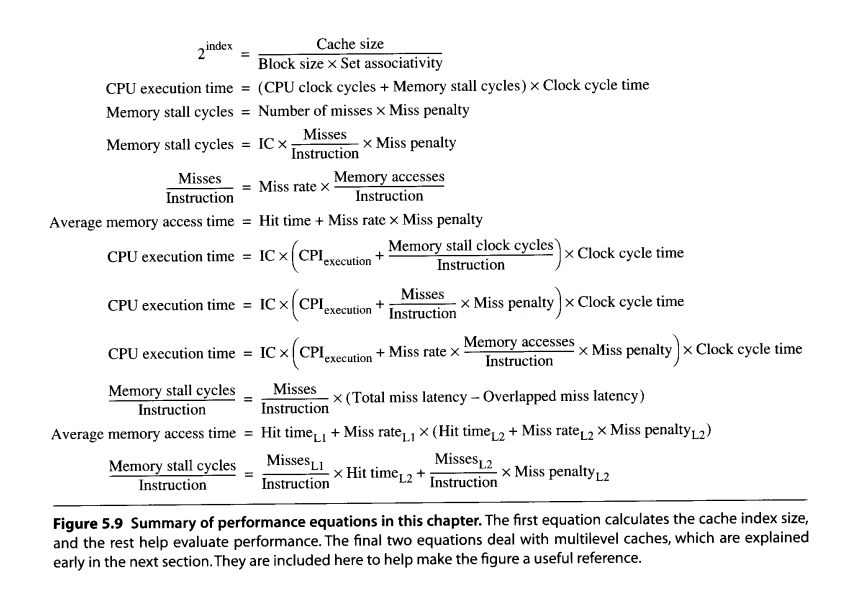
\includegraphics[width=\linewidth]{imagenes/ResumenPerformance.png}
\end{figure}


\section{Herramientas de modelado y analisis}

\subsection{Modelo 3C}
Es un modelo que permite buscar las fuentes de fallos en una jerarquia de memoria  y ver como los cambios en la jerarquia repercuten en la tasa de fallos.
Este modelo clasifica los cache misses en tres tipos:
\begin{itemize} 
    \item \textit{Fallos inevitables (Compulsory misses)} - Estos son los fallos de cache causados por el primer acceso a un bloque que nunca ha estado en la cache. Tambien se llaman fallos de arranca en frio (cold start misses). Es el miss rate de una cache LRU de tamaño infinito.
    \item \textit{Fallos de capacidad (Capacity misses)} - Estos son fallos cuando la cache no puede alocar todos los bloques necesarios para la ejecución de un programa. Los fallos de capacidad ocurre porque los bloques reemplazados son accedidos mas tarde. Es el miss rate de una cache LRU full associative menos el miss rate de una cache LRU full associative de tamaño infinito.
    \item \textit{Fallos de conflicto (Conflict misses)} - Estos occuren en cache asociativas o de mapeo directo, cuando multiples bloques compiten por una misma ubicación. Los fallos de conflictos son eliminados por una cache totalmente asociativa del mismo tamaño. Tambien se llaman fallos por colisión. Es el miss rate de la cache bajo estudio \textit{menos} el miss rate de una cache LRU full associative del mismo tamaño. 
\end{itemize}

\newpage
\begin{figure}[h!]
    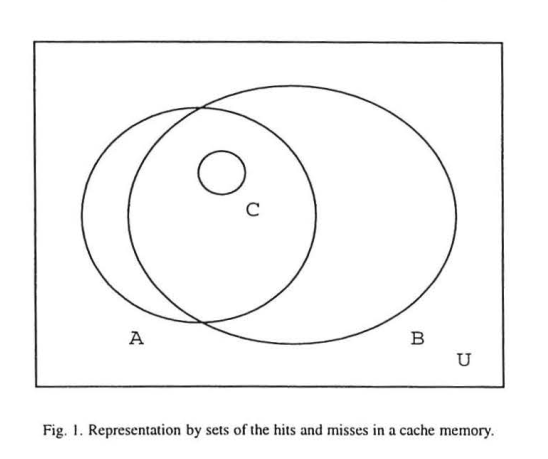
\includegraphics[width=\linewidth]{imagenes/Conjuntos3C.png}
\end{figure}

Donde \textit{U} es el conjunto de todas las referencias a memoria hechas por el programa, \textit{B} es el conjunto de referencias a memoria que dieron miss en la cache bajo analisis, 
\textit{A} es el conjunto de referencias que dieron miss en una cache full associative del mismo tamaño que la cache bajo analisis y usando una politica de reemplazo LRU y C es el conjunto que corresponde a las referencias a memoria en una cache de tamaño infinito.

\begin{align*}
    Compulsory &= \#C \\
    Capacity &= \#A - \#C \\
    Conflict &= \#B - \#A
\end{align*} 

Donde \#C, \#A y \#B es el numero de elementos en los conjuntos C, A y B respectivamente. 
Es sabido que en algunos casos es posible obtener valores negativos de miss rate de conflicto. Estos casos aparecen cuando una cache set associative tiene un miss rate mas chico que una cache full associative \(\#A > \#B\). 

El caracter estatico de este modelo no permite la clasificación individuales de los misses de memoria.

\subsection{Modelo D3C: Deterministic 3C model}
Se presenta una nueva definición para los tipos de misses. Para la correspondiente definición operacional se utiliza un politica de reemplazo LRU basado en distancias.

\begin{itemize} 
    \item \textit{Fallos inevitables (Compulsory misses)} - Un miss compulsivo es una referencia a memoria que da misses en la cache bajo analisis y tambien da misses en una cache LRU full associative de tamaño infinito.
    \item \textit{Fallos de capacidad (Capacity misses)} - Un miss de capacidad es una referencia a memoria que no da misses compulsivos en la cache bajos analisis y que tambien produce misses en una cache LRU full associative del mismo tamaño.
    \item \textit{Fallos de conflicto (Conflict misses)} - El resto de los misses no compulsivos son definidos como misses de conflicto.
\end{itemize}

\begin{align*}
    Compulsory &= C \\
    Capacity &= (A \cap B) - C \\
    Conflict &= B - A
\end{align*} 
Las operaciones son realizadas mediante conjuntos y por lo tanto los misses son clasificados de forma individual.

\subsection{Reducción de tasa de misses}

\begin{itemize}
    \item Cache mas grandes y asociativas. Las organizaciones de correspondencia directa sufren trashing. \textit{El esquema asocitivo por conjunto los reduce o elimina}.
    \item Bloques mas grandes.
    \item Reducción de ciclos de stall via paralelismo. Utilizando caches nos bloqueantes, hardware de prefeching, software de prefeching.
    \item Optizaciones del software
    \begin{enumerate}
        \item Lectura adelantada(prefeching): Especula los accesos futuros a datos e instrucciones. Desenrrollar el bloque para no ejecutar el prefeching en todas las iteraciones.
        \item Remplazo de elementos de arreglos: Remplazar el elemento de un arreglo por una variable temporal, para que pueda mantenerse en un registro.
        \item Intercambio de bucles: Según el lenguaje, un arreglo multidimencional podria almacenarse en memoria ordenado por filas o columnas.
        \item Operación el bloques: En una multiplicación de matrices hay una elevada cantidad de desaciertos. La solución es operar en bloques mas peques para que puedan ser mantenidos en cache.
        \item Rellenado de registros(padding): Se cambia la forma en que los arreglos son almacenados en memoria para que puedan ubicarse en filas distintas de la cache. Reduce los accesos conflictivos. Disminuye el trashing y por ende la cantidad de deshaciertos.
    \end{enumerate}
\end{itemize}

\subsection{Reducción de tiempo de hit}
\begin{itemize}
    \item Caches mas pequeñas y mas simples
    \item Evitar traducción de páginas
    \item Cache pipeline
    \item Trace cache
    \item Mejorar el ancho de banda de la memoria principal
    \begin{enumerate}
        \item One-word-wide memory organization
        \item Wide memory organization
        \item Interleaved memory organization: intercalando
        \item Tecnologia DRAM: Dinamic Random Access Memory
        \begin{enumerate}
            \item DRAM Convencional
            \item Fast Page Mode DRAM (FPM DRAM)
            \item Extended Data Out DRAM (EDO RAM)
            \item Synchronous DRAM (SDRAM)
        \end{enumerate}
        \item Evolución DRAM sincronica
        
    \end{enumerate}
    
\end{itemize}


\newpage
\section{Memoria Virtual}

En una computadora para un instante de tiempo pueden ejecutarse multiples procesos, cada uno con su propio espacio de memoria. Muchos procesos usan solo una pequeña parte de su espacio de direcciones. 
La memoria virtual, divide la memoria fisica en bloques y los aloca para diferentes procesos. Intrincecamente se puede intepretar como un esquema de proteccion para que un proceso este restringido solo a sus bloques alocados.
Tambien reduce el tiempo de arranque de los programas, desde que no se necesita que todo el código y datos esten en la memoria fisica.

La memoria virtual maneja de manera automatica los dos niveles de jeraquia de memoria representados por la memoria principal y los dispositivos de almacenamiento secuendarios.

\begin{figure}[h!]
    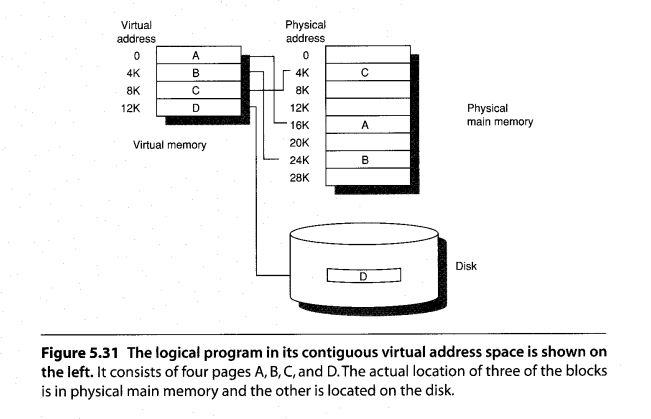
\includegraphics[width=\linewidth]{imagenes/VirtualAdress.png}
\end{figure}

\begin{quote}
    La memoria virtual implementa la traducción del espacio de direcciones de un programa a direcciones fisicas. Este proceso de traducción asegura del espacio de direcciones de un programa de otros.
    Ademas permite que un simple programa de usuario exceda el tamaño de la memoria principal
\end{quote}

Ademas de proveer protección para la memoria comportida y el manejo automatico de la jerarquia de memoria, tambien simplifica la carga de programas para su ejecución.
Llamamos \textit{relocación} al mecanismo que permite que el mismo programa se ejecuté en cualquier locación de la memoria fisica.

Varias ideas extraidas de la jeraquia de memorias con caches se pueden aplicar analogamente a memorias virtuales, aunque los terminos sean diferentes.
Las paginas (\textit{pages}) o segmentos (\textit{segment}) serian los bloques, y los \textit{fage fault} o \textit{address fault} actuarian como un miss. 
Con memoria virtual, la CPU produce \textit{direcciones virtuales}, las cuales son traducidas mediante una combinación de hardware y software a \textit{direcciones fisicas}. Este proceso se llama \textit{memory mapping} o \textit{address translation}.


\begin{figure}[h!]
    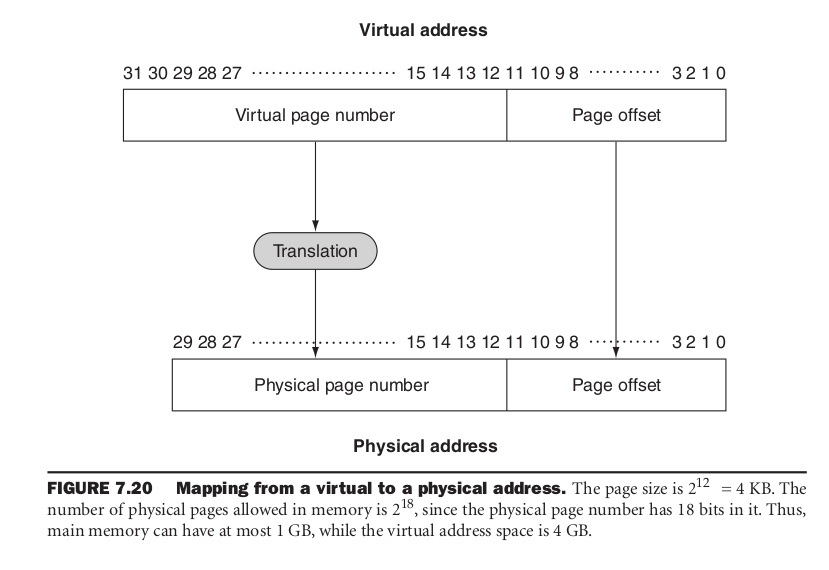
\includegraphics[width=\linewidth]{imagenes/TraduccionMemoriaVirtual.png}
\end{figure}


Hay mas diferencias entre caches y la memoria virtual:

\begin{enumerate}
    \item El reemplazo ante un cache miss es controlado principalmente por hardware, mientras que la memoria virtual el reemplazo es controlado principalmente mediante el sistema operativo. 
    \item El tamaño de direcciones del procesador determina el tamaño de la memoria virtual, pero el tamaño de la cache es independiente del tamaño de direcciones del procesador.
\end{enumerate}

\begin{figure}[h!]
    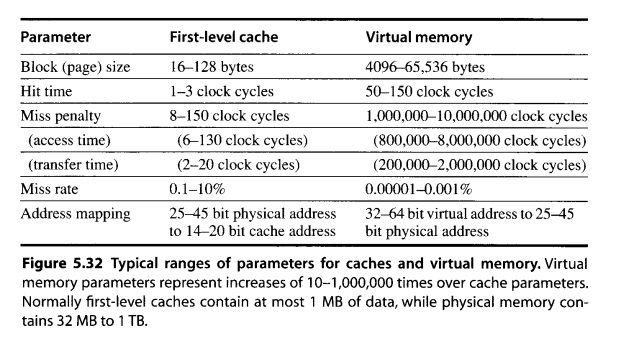
\includegraphics[width=\linewidth]{imagenes/VirtualAdressVsCache.png}
\end{figure}

Existen dos categorias de memoria virtual. Bloques de tamaño fijo llamados \textit{paginas} ó \textit{pages} y Bloques de tamaños variable llamados \textit{segmentos} o \textit{segment}

\begin{figure}[h!]
    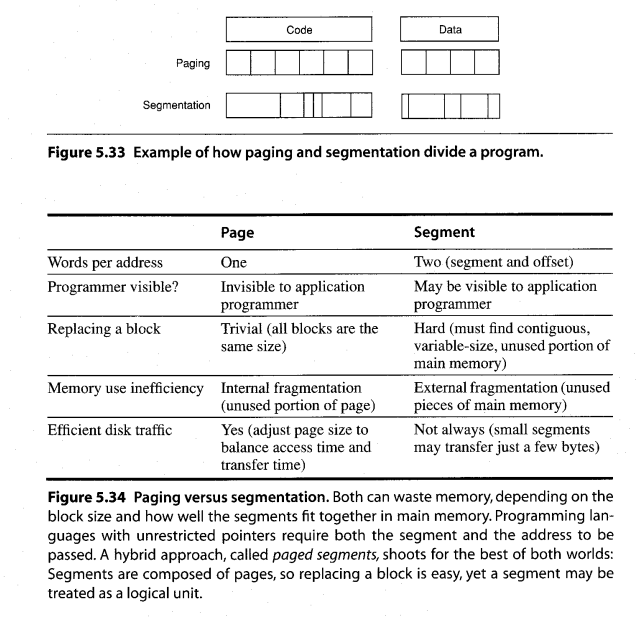
\includegraphics[width=\linewidth]{imagenes/PaginasVsSementos.png}
\end{figure}

\newpage
\subsection{Cuatro preguntas sobre Jerarquia de Memoria}
\subsubsection{¿Donde puede ubicarse los bloques en la memoria principal?}

El sistema operativo permite que los bloques puedan ser situados en cualquier lugar en la memoria principal.

\subsubsection{¿Como es encontrado un bloque si este esta en memoria principal?}

En ambos casos, paginado o segmentacion, se confia en la estructura de datos que esta indexada por la \textit{page number} o \textit{segment number}. Esta estructura de datos contiene la \textit{dirección fisica del bloque}.
En segmentacion, el offset es adicionado a la dirección fisica del segmento para obtener la dirección fisica final. En el caso del paginado, el offset es concatenado a la dirección de la pagina fisica (\textit{physical page address o physical page number - PPN}).

\begin{figure}[h!]
    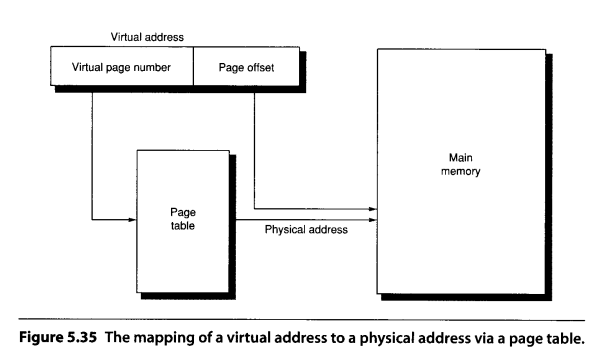
\includegraphics[width=\linewidth]{imagenes/MapeoMemoriaVirtual.png}
\end{figure}

La estructura de datos contiene el \textit{physical page address} que se obtiene de la \textit{page table}. Indexada por la \textit{virtual page number o VPN} el tamaño de la tabla es el numero de paginas en el espacio de memoria virtual.

Para reducir el tiempo de traducción, las computadores utilizan un cache dedicada para la traducción de direcciones, llamada \textit{translation lookaside buffer o TLB}.

\newpage
\subsubsection{¿Que bloque debe ser reemplazado ante un miss de memoria virtual?}

Casi todos los sistemas operativos tratan de reemplazar el bloque menos recientemente usado (LRU). Para estimar el LRU muchos procesadores proveen un \textit{bit de uso} o \textit{bit de referencia}, el cual se setea logicamente cuando una pagina es accedida.
El sistema operativo limpia de forma periodica el bit de uso que luego son escritos mas tarde, y entonces con esto se pueden determinar cuales paginas fueron accedidas durante un periodo de tiempo particular. De esta forma, el sistema operativo puede seleccionar una pagina de entre los menos recientemente usados(LRU).

\subsubsection{¿Que pasa ante una escritura?}

La estrategia de escritura es simpre Wirte Back. La memoria virtual incluye un \textit{dirty bit}. Este bit permite que los bloques sean escritos a disco solo si estos tuvieron cambios desde que fueron leidos desde disco.

\newpage
\subsection{Técnicas para una rapida traducción de direcciones}

Las tablas de paginas usualmente son tan largas que son guardadas en memoria principal y hasta incluso son paginas por ellas mismas. Paginar significa que cada acceso a memoria se hace dos veces, con un acceso a memoria se obtiene la dirección fisica y con un segundo acceso se obtiene el dato.

Solución, recordar la ultima traducción y de esta forma evitar el proceso de traducción si la dirección que se quiere referencias es la misma pagina que se accedio como la última.

Si se mantiene al direccion traducida en una cache especial, un acceso a memoria rara vez requerira un segundo acceso a memoria para traducir el dato. Esta cache especial es la \textit{TLB} o \textit{translation lookaside buffer}

Una entrada en la TLB es muy parecida a una entrada de cache. El Tag es una porcion de la memoria virtual y la porcion de data que mantiene es la \textit{physical page number}, \textit{protection field}, \textit{valid bit}, y tambien un \textit{use bit} y \textit{dirty bit}.

Notar que \textit{bit de dirty} corresponde a que la pagina esta sucia o dirty, no coorresponde a la traducción en entrada en la TLB.

\begin{figure}[h!]
    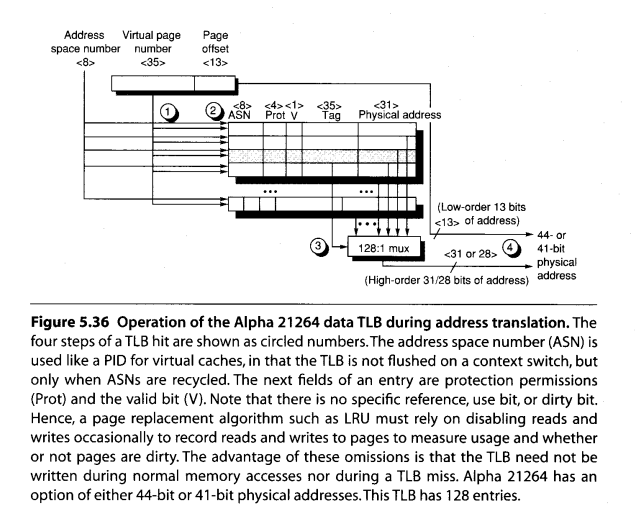
\includegraphics[width=\linewidth]{imagenes/TLB.png}
\end{figure}

Para reducir los TLB Misses debido al \textit{context switch} cada entrada tiene 8 bits para el \textit{address space number o ASN}. Si el context swiching retorna al proceso con el mismo ASN, este aun puede macheear con la TLB. Asi el proceso ASN y la page table entry deberían tambien machear con un tag valido.

No es neceario incluir los 13 bit del page offset. El page offset luego es combinado con el \textit{physical page frame} para formar la dirección fisica entera.


\newpage
\subsection{Cache direccionada fisicamente}

La cache esta fisicamente indexada y fisicamente tagueada. Todas las direcciones de memoria deben ser traducidas a direcciones fisica antes de acceder a la cache.
Se asume un tamaño de pagina de 4 KB, pero en realidad es de 16 KB. 

\begin{figure}[h!]
    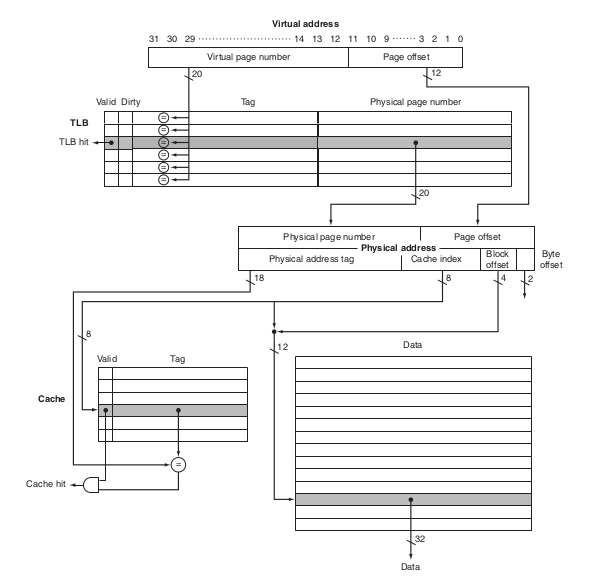
\includegraphics[width=\linewidth]{imagenes/CacheDireccionamientoFisico.png}
\end{figure}

\newpage
\subsection{Cache vitualmente indexada y fisicamente tagueada}

Ejemplo de traducción una dirección virtual de 64 bits a una dirección fisica de 41 bits con dos niveles de cache.
Mientras que la TLB es full asociativa, la cache es de mapeo directo. Para implementar un TLB full asociativa, se requiere que todos los TLB Tag sea comprado con el \textit{virtual page number} dado que puede estar en cualquier lugar de la TLB.
Si el bit de validez de la entrada que macheo, el acceso a la TLB es un hit y los bit de la PPN (\textit{physical page number}) junto con los bits del \textit{page offset} forman el indice para acceder a la cache.

\begin{figure}[h!]
    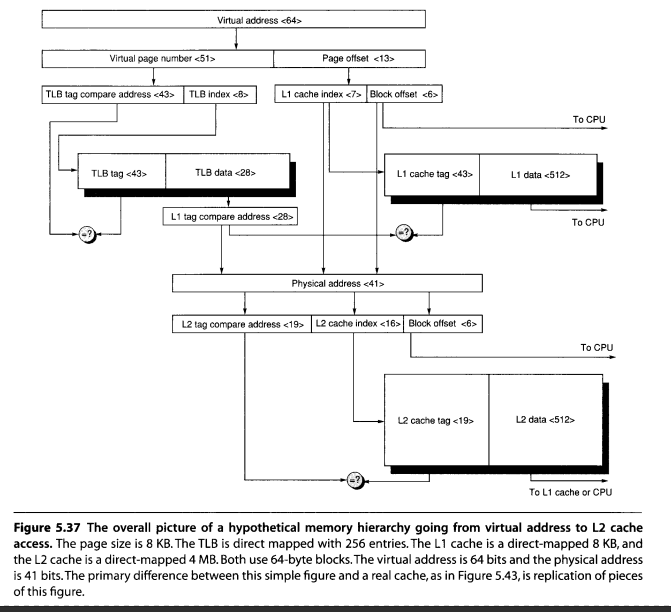
\includegraphics[width=\linewidth]{imagenes/CacheVirtualIndexadoTagFisico.png}
\end{figure}

La cache L1 esta virtualmente indexada y fisicamente tagueada desde que ambos tamaños de cache y tamaño de paginas son de 8 KB. La cache L2 es de 4MB. Ambas caches usan bloques de 64 bytes (512 bits). 

La dirección virtual se divide logicamente entre una \textit{Virtual Page Number} y \textit{Page Offset}. El primero es enviado a la TLB para ser traducida en una \textit{dirección fisica} y la segunda parte es enviada a la cacha L1 para ser utilizada como un indice.
Si la TLB machea con un hit, la \textit{physical page number} es enviado a la cache L1 para comparar si coincide con el \textit{L1 cache tag}. Si coincide, se produce un hit en la cache L1. El \textit{block offset} es enviado para seleccionar la palabra \textit{(word)} en la CPU.

Si el resultado de chequear el tag en cache L1 es un miss, la dirección fisica es usado en la cache L2. La parte el medio de la dirección fisica se utiliza como indice y la parte superior es comparado con tag de cache L2 seleccionado con el indice. Si coincide con el tag, entonces se produce un L2 cache hit, y el L2 data es enviado a la CPU, que junto con el offset se selecciona la palabra deseada.
Ante un cache miss en L2, la dirección fisica es utilizada para obtener el bloque de memoria.

\subsection{Arquitectura multihilo}

\textit{Multithreading} permite que multiples hilos compartan las unidades funcionales de un procesador simple de forma solapada. Para que puedan compartirse, el procesador debe duplicar el estado de cada hilo.
Por ejemplo, una copia separada del register file, un PC separado, y una tabla de paginas separada para cada hilo.
La memoria puede ser compartida mediante el mecanismo de la memoria virtual, el cual ya soporta multiprogramación.
Ademas, el hardware debe poder tener la habilidad de poder cambiar a un hilo diferente relativamente rapido. Un thread switch debe ser mas rapido que un context switch de un procesador.

Hay dos aproximaciones de multihilos, \textit{Fine-grained Multithreading(FMT)} cambia entre hilos en cada instrucción, intercalando asi la ejecución de multiples hilos. Para intercarlar hilos se utiliza round-robin, saltando los hilos que esten en stall. Para que sea practico, el CPU debe poder cambiar de hilo en cada ciclo de reloj.
Una ventaja es que se puede ocultar la perdida throughput de tanto stall largos como cortos, ejecutando instrucciones de otro hilo mientras un hilo este en stall. 
La principal desventaja es que se demora la ejecución de hilos individuales, debido a que si un hilo que no esta en stall, debe esperar a que se terminen de ejecutar intrucciones de otros hilos.

\textit{Coarse-grained Multithreading(CMT)} Solo cambia de hilo cuando un stall es muy costoso. Esta limitado su capacidad de obtener bajo throughput, especialmente en stall cortos.

Simultaneous multithreading (SMT)


\section{Un viaje de Arquitectura de conjunto de instrucciones (ISA)}

\subsection
    Es un producto de diferentes grupos que se involucraron en la arquitectura durante 20 años.
    \begin{enumerate}
        \item 1985 -  El 80386 extiende la arquitectura de 80286 a 32 bits. Ademas de agregar una arquitectura de 32 bits con registros de 32bits y un espacio de direcciones de 32 bits, agrega nuevos modos de direccionamiento y operaciones adicionales.
    \end{enumerate}

\end{document}

